\documentclass[fleqn]{jbook}
\usepackage{physpub}
\usepackage[dvipdfm]{graphicx}
\usepackage{amsmath}
\usepackage{amscd}
\usepackage{amssymb}
\usepackage{wrapfloat}
\usepackage{subfigure}
\setlength{\columnsep}{3zw}
%\setlength{\columnseprule}{0.4pt}
\if01 % by Murase
  % \thesection は physpub で \hspace{-1zw} に上書きされている。
  % 本来の \thesection を使いたければ、\Thesection に退避されている物を使用。
  \renewcommand{\theequation}{\thesection.\arabic{equation}}
  \renewcommand{\thefigure}{\thesection.\arabic{figure}}
  \renewcommand{\thetable}{\thesection.\arabic{table}}
  \numberwithin{equation}{section}
  \numberwithin{figure}{section}
  \numberwithin{table}{section}
\fi
%\renewcommand{\figurename}{Fig}
\usepackage[usenames]{color}


\begin{document}

\begin{question}{第2問}{}
% 問題はM.Yが入力しました。

金属中の伝導電子系をフェルミ・ディラック統計に従う自由電子気体とみなす単純なモデルを考える。
図\iref{2004phy2-0}に示したように、金属内部を表す一辺$L$の立方体の箱の中はポテンシャルがゼロで、外部は$V(>0)$になっているものとする。
この中に$N$個の電子が存在する。このとき以下の設問に答えよ。
ただし、電子の質量を$m$、ボルツマン定数を$k_B$、$\hbar=h/(2\pi)$($h$はプランク定数)とする。
なお、設問2以降では、$L$および$N$が十分に大きいとし、エネルギー準位の分布はほぼ連続と見なして良い。

\begin{enumerate}
\item $V$が十分に大きいものとし、波動関数$\psi(x,y,z)$に周期的境界条件
  $$
  \psi(x+L,y,z)=\psi(x,y,z), ~~\psi(x,y+L,z)=\psi(x,y,z),~~\psi(x,y,z+L)=\psi(x,y,z),
  $$
  を適用することによって、箱の中の電子状態を表す固有関数と固有エネルギーを求めよ。
\item 状態密度$g(\epsilon)$を求めよ。状態密度とは、エネルギーが$\epsilon$と$\epsilon+d\epsilon$の範囲にある単位体積あたりの電子状態の数を$g(\epsilon)d\epsilon$と表したときの$g(\epsilon)$である。

\item 温度$T=0$における化学ポテンシャル(フェルミ準位)$\mu_0$と、電子の数密度$n=N/L^3$との関係を求めよ。

\item 温度$T>0$では高いエネルギー状態にも有限の確率で電子が分布するので、一部の電子は表面から外部(真空中)に飛び出すことができる。表面に垂直で外向きの方向を$+z$軸として、単位面積から単位時間に外部に流れ出す電子の数$J_n$を、フェルミ分布関数$f(\epsilon)$、電子の$z$方向の速度$v_z$を含む三次元波数空間での積分をして表せ。その際、三次元波数空間の積分範囲を明示せよ。

\item $k_B T \ll(V-\mu)$(ただし$\mu$は有限温度での化学ポテンシャル)という近似のもとで設問4の積分を実行することにより、表面から単位時間、単位面積あたりに外部に流れ出す電子の数が
  $$
  J_n=\frac{4\pi m(k_B T)^2}{(2\pi \hbar)^3}\exp\left(
  -\frac{V-\mu}{k_B T}
  \right)
  $$
  となることを示せ。
\end{enumerate}


\begin{figure}[htbp]
\begin{center}
%\includegraphics[scale=0.5]{2004phy2-0.eps}
\includegraphics[width=10cm]{2004phys2_0.eps}
\caption{}
\eqname{2004phy2-0}
\end{center}
\end{figure}
\end{question}

\begin{answer}{第2問}{}
\begin{enumerate}
\item
  箱の中の Schr\"{o}dinger eq.は
  \begin{equation}
  -\frac{\hbar^2}{2m}\bigtriangleup \psi =E\psi\eqname{eq:16}
  \end{equation}
  $\psi$を変数分離して$\psi=X_1(x)X_2(y)X_3(z)$として式~(\eqhref{eq:16})に代入し,
  $\psi$でわると
  \begin{equation}
   -\frac{\hbar^2}{2m}\left(\frac{X_1''(x)}{X_1(x)}+\frac{X_2''(y)}{X_2(y)}+\frac{X_3''(z)}{X_3(z)}\right)=E\eqname{eq:17}
  \end{equation}
  左辺の第1項,第2項,第3項は定数である必要があり,それぞれ
  $E_1,E_2,E_3(>0)$とおくと式~(\eqhref{eq:17})は
  \begin{align}
  -\frac{\hbar^2}{2m}X''_i &=E_i X_i \nonumber \\ 
  k_i^2&\equiv \frac{2mE_i}{\hbar^2}\nonumber
  \end{align}
  とおくと
  \begin{equation}
   X_1(x)=e^{ik_1x},X_2(y)=e^{ik_2y},X_3(z)=e^{ik_3z}
  \end{equation}
  よって波動関数は
  \begin{equation}
   \psi=e^{i(k_1x+k_2y+k_3z)}\eqname{eq:18}
  \end{equation}
  規格化すると
  \[
   \int_{\text{BOX}}d^3x \psi^{\ddagger}\psi =L^3
  \]より
  \begin{equation}
   \psi=\frac{1}{\sqrt{L^3}}e^{i(k_1x+k_2y+k_3z)} \eqname{eq:20}
  \end{equation}
  ただし,周期的境界条件より波数の満たす条件は
  $X_i(\xi+L)=X(\xi)\,\,(\xi=x,y,z)$
  \begin{equation}
   ∴\,\,e^{ik_i L}=1 \Rightarrow \,\, k_i L=2\pi n_i \,\,\,\,(n_i\in
   \textbf{Z}) \eqname{eq:100}
  \end{equation}
  固有エネルギーは
  \begin{align}
   E&=E_1+E_2+E_3\nonumber\\
  &=\frac{\hbar^2}{2m}(k_1^2+k_2^2+k_3^2)=\frac{\hbar^2}{2m}\left(\frac{2\pi}{L}\right)^2 (n_1^2+n_2^2+n_3^2)\eqname{eq:19}
  \end{align}

\item
  ~(\eqhref{eq:100})より,波数空間では状態数は一辺$(2\pi/L)$の格子状に分布している.
  このとき半径$[k,k+dk]$の間に含まれる状態数を数えると,スピンの自由度に
  気をつけて
  \begin{equation}
  2 \times \frac{4\pi k^2 dk}{(2\pi/L)^3}=L^3g(\epsilon)d\epsilon \eqname{eq:21}
  \end{equation}
  $\epsilon=k^2\hslash^2/2m$より$k dk= m/\hslash^2 d \epsilon$であるから式~
  (\eqhref{eq:21})の左辺は
  \begin{equation}
   2 \times \frac{4\pi k^2 dk}{(2\pi/L)^3}=\frac{4\pi L^3}{h^3}(2m)^{3/2}\epsilon^{1/2}d\epsilon
  \eqname{eq:22}
  \end{equation}
  \begin{equation}
   ∴\,\, g(\epsilon)=\frac{4 \pi }{h^3}(2m)^{3/2}\epsilon^{1/2}\eqname{eq:23}
  \end{equation}

\item
  電子数密度は
  \begin{equation}
   n=\frac{N}{L^3}=\int_{0}^{\infty}d\epsilon g(\epsilon)f(\epsilon)\eqname{eq:24}
  \end{equation}
  とかける.ここで$f(\epsilon)$はFermi分布関数であり
  \[
   f(\epsilon)=\frac{1}{e^{\beta(\epsilon-\mu)}+1}
  \]
  である.今$T=0$であるから$\beta\rightarrow \infty$であり分布関数は図~\iref{fig:fermi}のよう
  になる
  \begin{figure}[htbp]
   \begin{center}
  \resizebox{!}{5cm}{%WinTpicVersion3.08
\unitlength 0.1in
\begin{picture}( 33.1000, 21.1000)(  6.9000,-24.0000)
% VECTOR 2 0 3 0
% 4 800 2200 4000 2200 1000 2400 1000 400
% 
\special{pn 8}%
\special{pa 800 2200}%
\special{pa 4000 2200}%
\special{fp}%
\special{sh 1}%
\special{pa 4000 2200}%
\special{pa 3934 2180}%
\special{pa 3948 2200}%
\special{pa 3934 2220}%
\special{pa 4000 2200}%
\special{fp}%
\special{pa 1000 2400}%
\special{pa 1000 400}%
\special{fp}%
\special{sh 1}%
\special{pa 1000 400}%
\special{pa 980 468}%
\special{pa 1000 454}%
\special{pa 1020 468}%
\special{pa 1000 400}%
\special{fp}%
% LINE 2 0 3 0
% 4 1000 1000 2800 1000 2800 1000 2800 2200
% 
\special{pn 8}%
\special{pa 1000 1000}%
\special{pa 2800 1000}%
\special{fp}%
\special{pa 2800 1000}%
\special{pa 2800 2200}%
\special{fp}%
% STR 2 0 3 0
% 3 960 900 960 1000 4 0
% $1$
\put(9.6000,-10.0000){\makebox(0,0)[rt]{$1$}}%
% STR 2 0 3 0
% 3 960 2140 960 2240 4 0
% $0$
\put(9.6000,-22.4000){\makebox(0,0)[rt]{$0$}}%
% STR 2 0 3 0
% 3 2760 2140 2760 2240 4 0
% $\mu_0$
\put(27.6000,-22.4000){\makebox(0,0)[rt]{$\mu_0$}}%
% STR 2 0 3 0
% 3 3960 2140 3960 2240 1 0
% $\epsilon$
\put(39.6000,-22.4000){\makebox(0,0)[lt]{$\epsilon$}}%
% STR 2 0 3 0
% 3 1090 360 1090 460 2 0
% $f(\epsilon)$
\put(10.9000,-4.6000){\makebox(0,0)[lb]{$f(\epsilon)$}}%
\end{picture}%
}
   \end{center}
  \caption{Fermi Distribution Function}
  \eqname{fig:fermi}
  \end{figure} 
  電子はFermiポテンシャル以下の状態に収まっており式~(\eqhref{eq:24})は以下の
  ようになる.
  \begin{align*}
   n&=\int_{0}^{\mu_0}d\epsilon g(\epsilon)=\int_{0}^{\mu_0}d\epsilon \frac{4\pi }{h^3}(2m)^{3/2}\epsilon^{1/2}\\
  &=\frac{8\pi }{3h^3}(2m)^{3/2}\mu_0^{3/2}
  \end{align*} 
\item
  電子が飛び出す条件は$v_z(>0)$が

  \begin{equation}
   \frac{1}{2}mv_z^2>V \eqname{eq:27}
  \end{equation}

  であることである.$v_z$がこの条件を満たすとき,$J_n$は題意により図~\iref{fig:tyo}の直方
  体の中に含まれる電子の総数に等しい.
  \begin{figure}[h]
  \begin{center}
   %WinTpicVersion3.08
\unitlength 0.1in
\begin{picture}(  6.4000, 12.4000)( 20.0000,-24.4000)
% LINE 2 0 3 0
% 22 2200 2200 2000 2400 2000 2400 2000 1400 2000 1400 2200 1200 2200 1200 2600 1200 2600 1200 2400 1400 2400 1400 2000 1400 2400 1400 2400 2400 2400 2400 2000 2400 2400 2400 2600 2200 2600 2200 2200 2200 2600 2200 2600 1200
% 
\special{pn 8}%
\special{pa 2200 2200}%
\special{pa 2000 2400}%
\special{fp}%
\special{pa 2000 2400}%
\special{pa 2000 1400}%
\special{fp}%
\special{pa 2000 1400}%
\special{pa 2200 1200}%
\special{fp}%
\special{pa 2200 1200}%
\special{pa 2600 1200}%
\special{fp}%
\special{pa 2600 1200}%
\special{pa 2400 1400}%
\special{fp}%
\special{pa 2400 1400}%
\special{pa 2000 1400}%
\special{fp}%
\special{pa 2400 1400}%
\special{pa 2400 2400}%
\special{fp}%
\special{pa 2400 2400}%
\special{pa 2000 2400}%
\special{fp}%
\special{pa 2400 2400}%
\special{pa 2600 2200}%
\special{fp}%
\special{pa 2600 2200}%
\special{pa 2200 2200}%
\special{fp}%
\special{pa 2600 2200}%
\special{pa 2600 1200}%
\special{fp}%
% STR 2 0 3 0
% 3 2170 2340 2170 2440 1 0
% $1$
\put(21.7000,-24.4000){\makebox(0,0)[lt]{$1$}}%
% STR 2 0 3 0
% 3 2530 2220 2530 2320 1 0
% $1$
\put(25.3000,-23.2000){\makebox(0,0)[lt]{$1$}}%
% STR 2 0 3 0
% 3 2640 1620 2640 1720 1 0
% $v_z$
\put(26.4000,-17.2000){\makebox(0,0)[lt]{$v_z$}}%
% LINE 2 2 3 0
% 2 2200 1200 2200 2200
% 
\special{pn 8}%
\special{pa 2200 1200}%
\special{pa 2200 2200}%
\special{dt 0.045}%
\end{picture}%

  \end{center}
  \caption{単位体積から単位時間に流れ出す電子が含まれる}
  \eqname{fig:tyo}
  \end{figure}
  波数が$[k,k+dk]$にある単位体積あたりの電子状態の数は
  \[
   \frac{2}{(2\pi)^3}dk_xdk_ydk_z
  \]
  であるから
  \begin{align}
   J_n&=\int_{v_z>\sqrt{2V/m}}dk_z \int_{\textbf{R}}dk_x \int_{\textbf{R}}dk_y g(k)f(k) \nonumber\\
  &=\int_{v_z>\sqrt{2V/m}}dk_z \int_{\textbf{R}}dk_x \int_{\textbf{R}}dk_y \frac{2v_z}{(2\pi)^3}\nonumber\\
  & \times \frac{1}{\exp\left[\beta\left\{\frac{\hbar^2}{2m}(k_x^2+k_y^2+k_z^2)-\mu\right\}+1\right]} \eqname{eq:26} 
  \end{align}

\item
  (\eqhref{eq:27})より
  \begin{align*}
   \exp\left(\beta\left(\frac{\hbar^2k^2}{2m}-\mu\right)\right)&>\exp(\beta(V-\mu))\\
  \beta(V-\mu)\gg 1 &\Rightarrow \exp(\beta(V-\mu))\gg 1
  \end{align*}
  よって~(\eqhref{eq:26})の被積分関数の指数関数部分は

  \begin{align*}
  & \frac{1}{\exp\left[\beta\left\{\frac{\hbar^2}{2m}(k_x^2+k_y^2+k_z^2)-\mu\right\}+1\right]}\\
  &= \exp\left[-\beta\left\{\frac{\hbar^2}{2m}(k_x^2+k_y^2+k_z^2)-\mu\right\}\right]
  \end{align*}

  とかける.従って
  \begin{align*}
   J_n&=\int_{v_n>\sqrt{2v/m}}dk_z \int_{-\infty}^{\infty}dk_x \int_{-\infty}^{\infty}dk_y\frac{2v_z}{(2\pi)^3}\\
  &\times \exp\left[-\beta\left\{\frac{\hbar^2}{2m}(k_x^2+k_y^2+k_z^2)-\mu\right\}\right]\\
  &=\frac{4\pi}{(2\pi)^3}\cdot\frac{1}{\beta \hbar}\exp(\beta\mu)\int_{\sqrt{2mV/\hbar}}^{\infty}dk_z\exp\left[-\frac{\beta\hbar^2k^2_z}{2m}\right]\\
  &=\frac{4m\pi}{(2\pi \hbar)^3 \beta^2}\exp\{-\beta(V-\mu)\}
  \end{align*}
  とかける.

\end{enumerate}
\end{answer}
\end{document}
